\documentclass[t]{beamer}
\usetheme{Copenhagen}
\setbeamertemplate{headline}{} % remove toc from headers
\beamertemplatenavigationsymbolsempty

\usepackage{amsmath, array, tikz, bm, pgfplots, tcolorbox, graphicx, venndiagram, color, colortbl}
\pgfplotsset{compat = 1.16}
\usepgfplotslibrary{statistics}
\usetikzlibrary{calc}

\title{Quantitative Graphs}
\author{}
\date{}

\AtBeginSection[]
{
  \begin{frame}
    \frametitle{Objectives}
    \tableofcontents[currentsection]
  \end{frame}
}

\begin{document}

\begin{frame} 
\maketitle
\end{frame}

\section{Create a frequency distribution for quantitative data}

\begin{frame}{Frequency Distribution for Quantitative Data}
The weights (in pounds) of 25 husky dogs are shown below:
\begin{center}
\begin{tabular}{ccccc}
53 & 46 & 44 & 47 & 50 \\
49 & 47 & 44 & 61 & 44 \\
35 & 46 & 49 & 51 & 48 \\
50 & 52 & 44 & 50 & 47 \\
58 & 47 & 52 & 37 & 54 \\
\end{tabular}
\end{center}
Suppose we want to create a frequency distribution for the weights of these awesome dogs. \newline\\	\pause

Since this data is quantitative, we are going to have to decide what each of our ranges of weights in our classes is going to be. 
\end{frame}

\begin{frame}{Definitions for Quantitative Data}
The smallest value (weight in our case) in each class (table row) is called the {\color{blue}\textbf{lower class limit}}. \newline\\	\pause

The largest value in each class is the {\color{blue}\textbf{upper class limit}}. \newline\\ \pause 

Typically, the closer the lower and upper class limits are in value, the more classes we will need. \newline\\	\pause

The difference between two consecutive lower class limits is called the {\color{blue}\textbf{class width}}.	\newline\\	\pause

Let's create a frequency distribution for the dog weights using a class width of 5 pounds.
\end{frame}

\begin{frame}{Frequency Distribution of the Weights of Adorable Huskies}
\begin{center}
\begin{tabular}{c|c}
\textbf{Weight} & \textbf{Frequency} \\ \hline
35 -- 39 & 2 \\
40 -- 44 & 4 \\
45 -- 49 & 9 \\
50 -- 54 & 8 \\
55 -- 59 & 1 \\
60 -- 64 & 1 \\
\end{tabular}
\end{center}
\pause
In the above table, we are only considering integer weight values.	\newline\\	\pause

However, any dog that weighs more than 39.5 pounds, but less than 44.5 pounds, would have to go into the 40 -- 44 pound class. \newline\\	\pause

Going a half of another decimal place below the lower class limit and above the upper class limits give us the {\color{blue}\textbf{class boundaries}}.
\end{frame}

\section{Create and interpret histograms}

\begin{frame}{Histograms of Quantitative Data}
We can use class limits to create a histogram of the data.	\newline\\	\pause

A histogram is like a bar graph in which there are no gaps between classes.		\pause

\begin{center}
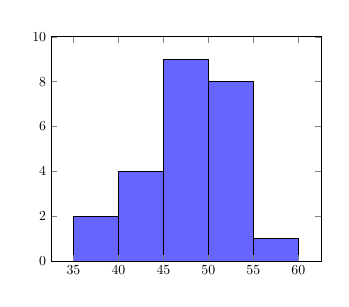
\begin{tikzpicture}[scale=0.5]
\begin{axis}[
ymin = 0, ymax = 10, area style
]
\addplot[ybar interval, fill=blue!60, mark=no] plot coordinates {(35,2) (40,4) (45,9) (50,8) (55,1) (60,1)};
\end{axis}
\end{tikzpicture}
\end{center}
\pause We can also use class midpoints when graphing histograms. \pause \newline\\

To find the class midpoint, add the lower class limit and upper class limit. Then divide by two.
\end{frame}

\begin{frame}{Example 1}
(a) \quad Given the histogram below of the weights of 200 dogs, find the total number of dogs whose weight is at least 34 pounds.	\newline\\
\begin{minipage}{0.7\textwidth}
\begin{tikzpicture}
\node at (0,0) {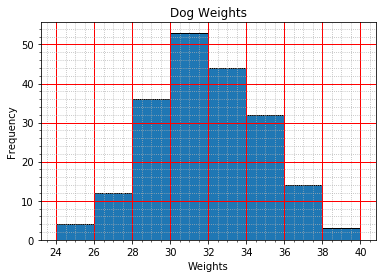
\includegraphics[scale=0.55]{../Images/dog_weights_hist.png}};
\onslide<2->{\node at (1.45,0.65) {32};}
\onslide<3->{\node at (2.15,-0.65) {14};}
\onslide<4->{\node at (2.9,-1.5) {3};}
\end{tikzpicture}
\end{minipage}
\hspace{0.25cm}
\begin{minipage}{0.2\textwidth}
\onslide<5->{Total: 49}
\end{minipage}
\end{frame}

\begin{frame}{Example 1}
(b) \quad What percentage of the dogs have weights between 26 and 28 pounds?	\newline\\
\begin{minipage}{0.7\textwidth}
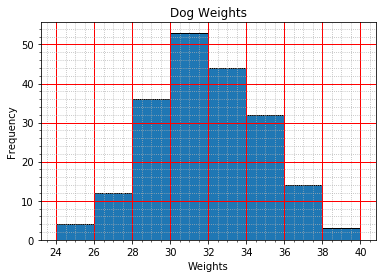
\includegraphics[scale=0.55]{../Images/dog_weights_hist.png}
\end{minipage}
\hspace{0.25cm}
\begin{minipage}{0.2\textwidth}
\onslide<2->{12/200} \\[10pt]
\onslide<3->{6\%}
\end{minipage}
\end{frame}

\begin{frame}{Relative Frequency Histogram}
We can even make a relative frequency histogram of a data set.	\newline\\	\pause

The total area of all rectangles will equal 100\%.	\newline\\	\pause
\begin{center}
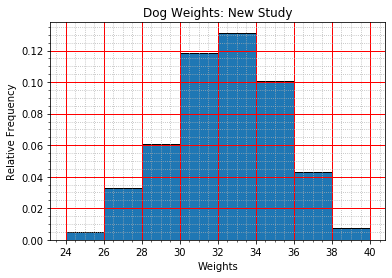
\includegraphics[scale=0.55]{../Images/dog_weights_relfreq_hist.png}
\end{center}
\end{frame}

\begin{frame}{Some Common Histogram Shapes}
Uniform distribution:	\newline\\
\begin{center}
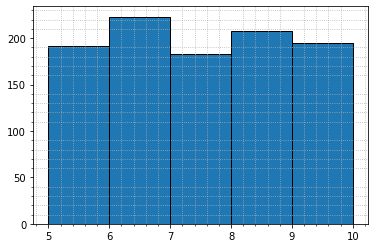
\includegraphics[scale=0.55]{../Images/uniform.png}
\end{center}
\end{frame}

\begin{frame}{Som Common Histogram Shapes}
Right (a.k.a. positively) skewed
\begin{center}
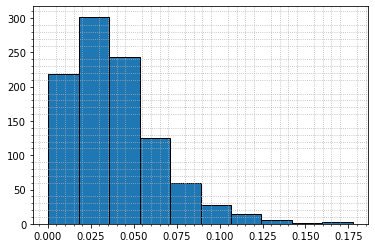
\includegraphics[scale=0.55]{../Images/positive_skewed.png}
\end{center}
\onslide<2->{\emph{Note}: Skewness refers to the \underline{tail}}
\end{frame}

\begin{frame}{Som Common Histogram Shapes}
Normal (a.k.a. bell-shaped)
\begin{center}
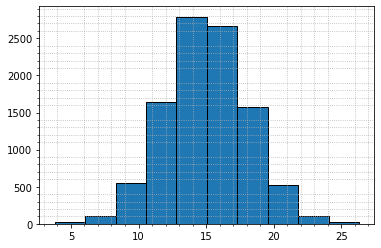
\includegraphics[scale=0.55]{../Images/normal1.png}
\end{center}
\end{frame}

\begin{frame}{Som Common Histogram Shapes}
Left (a.k.a. negatively) skewed
\begin{center}
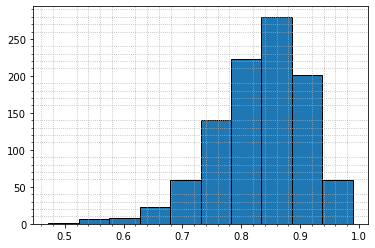
\includegraphics[scale=0.55]{../Images/negative_skewed.png}
\end{center}
\end{frame}

\end{document}